\section{Question 3}

\begin{verbatim}
Write a formal model of Clojure with core.spec, and implement it in
PLT Redex. Formulate a consistency property between contracted and
uncontracted execution, and test it in redex.
\end{verbatim}

\subsection{Formal model}

%\begin{figure*}
$$
\begin{altgrammar}
  \e{} &::=& \x{}
                      \alt \v{} 
                      \alt {\comb {\e{}} {\e{}}} 
                      \alt {\abs {\x{}} {\e{}}}
                      \alt {\ifexp {\e{}} {\e{}} {\e{}}}
                &\mbox{Expressions} \\
  \v{} &::=&          {\emptymap{}}
											\alt {\err{}}
                      \alt {\num{}}
                      \alt \mapval{}
                      \alt {\closure {\openv{}} {\abs {\x{}} {\e{}}}}
                &\mbox{Values} \\
  \mapval{} &::=&  {\curlymapvaloverright{\v{}}{\v{}}}
                &\mbox{Map Values} \\
\rho  &::=& [\overrightarrow{\x{} \mapsto \v{}}]
                &\mbox{Environments} \\
  p  &::=& \zerohuhliteral{} \alt \numberhuhliteral{} \alt \booleanhuhliteral{}
					%\alt \nilhuhliteral{}
                &\mbox{Predicates} \\
  c	 &::=&  p \alt \getliteral{} \alt \assocliteral{} &\mbox{Constants} \\
  \Ctxt &::=& [] \alt {\comb{\Ctxt}{\e{}}} \alt {\comb{\v{}}{\Ctxt}} \alt 
								{\ifexp {\Ctxt} {\e{}} {\e{}}}
                &\mbox{Contexts} \\

\end{altgrammar}
$$
\caption{Syntax of Terms in $\lambda c$}
\end{figure*}


We devise a base formal model for Clojure called \lambdac{}
(syntax defined in Figure~\ref{clojure-grammar}).
We extend \lambdac{} with clojure.spec with \texttt{fdef} but without 
\texttt{fspec} specs, and call
this model \lambdacs{}
(syntax defined in Figure~\ref{clojurespec-grammar}).
Then, we extend \lambdacs{} to support
\texttt{fspec} function contracts, and call this final model \lambdacsf{}
(syntax defined in Figure~\ref{clojurespechof-grammar}).

We define the small-step reduction rules for each language, using contexts.
Figure~\ref{arrowv} defines the reduction rules for 
the base language \lambdac{}---it does not include any spec features.
Figure~\ref{arrowvspec} defines the reduction rules for 
\lambdacs{}, adding support for \texttt{fdef}.
Finally, Figure~\ref{arrowvspec-hof} defines the reduction rules for 
\lambdacsf{}, adding support for \texttt{fspec}.

\subsection{Consistency property}

Let $\rightarrow^{*}$ be the reflexive, transitive closure of $\rightarrow$,
the single-step reduction relation for our respective languages.

We formulate two consistency properties, one which we expect to hold, another
which does not hold, and test them both using Redex.

The first theorem (Theorem~\ref{th1}) states that any expression in \lambdac{}
evaluates to the same value (or error) as checking that value against
any spec in \lambdacs{}, or throws a spec value.
For example, \texttt{1} in \lambdac{} evaluates to the same value (or error)
as \texttt{(assert-spec 1 number?)}. Furthermore, \texttt{(assert-spec 1 zero?)} 
evaluates to a spec error.

\begin{theorem}[Consistency without fspec]
\label{th1}
For every expression \texttt{E} in \lambdac{}, 
and every spec $\mathbb{S}$ in \lambdacs{}, 
if \texttt{E} $\rightarrow^{*}$ $\texttt{V}_1^{e}$ and
\texttt{(assert-spec E $\mathbb{S}$)} $\rightarrow^{*}$ $\texttt{V}_2^{e}$,
then either:
\begin{itemize}
\item $\texttt{V}_1^{e} = \texttt{V}_2^{e}$, or
\item $\texttt{V}_2^{e}$ is \texttt{(error spec-error ...)}.
\end{itemize}
\end{theorem}

We formulated Theorem~\ref{th1} in Redex, and tested it for 1000 expressions,
each with 1000 specs. We found no counter-examples, as expected.

We expect to find a counter-example in Theorem~\ref{th2}, however.
It is similar to Theorem~\ref{th1}, except we compare \lambdac{} with
\lambdacs{}, which includes \texttt{fspec}s (with generative testing semantics).

\begin{theorem}[Consistency with fspec]
\label{th2}
For every expression \texttt{E} in \lambdac{}, 
and every spec $\mathbb{S}$ in \lambdacsf{}, 
if \texttt{E} $\rightarrow^{*}$ $\texttt{V}_1^{e}$ and
\texttt{(assert-spec E $\mathbb{S}$)} $\rightarrow^{*}$ $\texttt{V}_2^{e}$,
then either:
\begin{itemize}
\item $\texttt{V}_1^{e} = \texttt{V}_2^{e}$, or
\item $\texttt{V}_2^{e}$ is \texttt{(error spec-error ...)}.
\end{itemize}
\end{theorem}

Formulating Theorem~\ref{th2} in Redex finds many counter-examples
involving \texttt{fspec}.
For example, the following call that generates only 10 expressions each with 10
random specs finds a ``stuck'' term from trying to generatively test a one-argument
function \texttt{boolean?} as if it had zero-arguments (there is no way to know
a function's arity in advance).

\begin{verbatim}
> (check-Clojure-ClojureSpecHOF-compat 10 10)
ERROR:
ClojureSpec evaluation did not fully reduce
Original-form: (assert-spec boolean? (FSpec () zero? 0))
Stuck-form: (assert-spec boolean? (FSpec () zero? 0))
\end{verbatim}

%\subsection{Redex model}

%We model \lambdac{} as a Redex language called \emph{Clojure}.

\begin{figure*}
\fbox{
  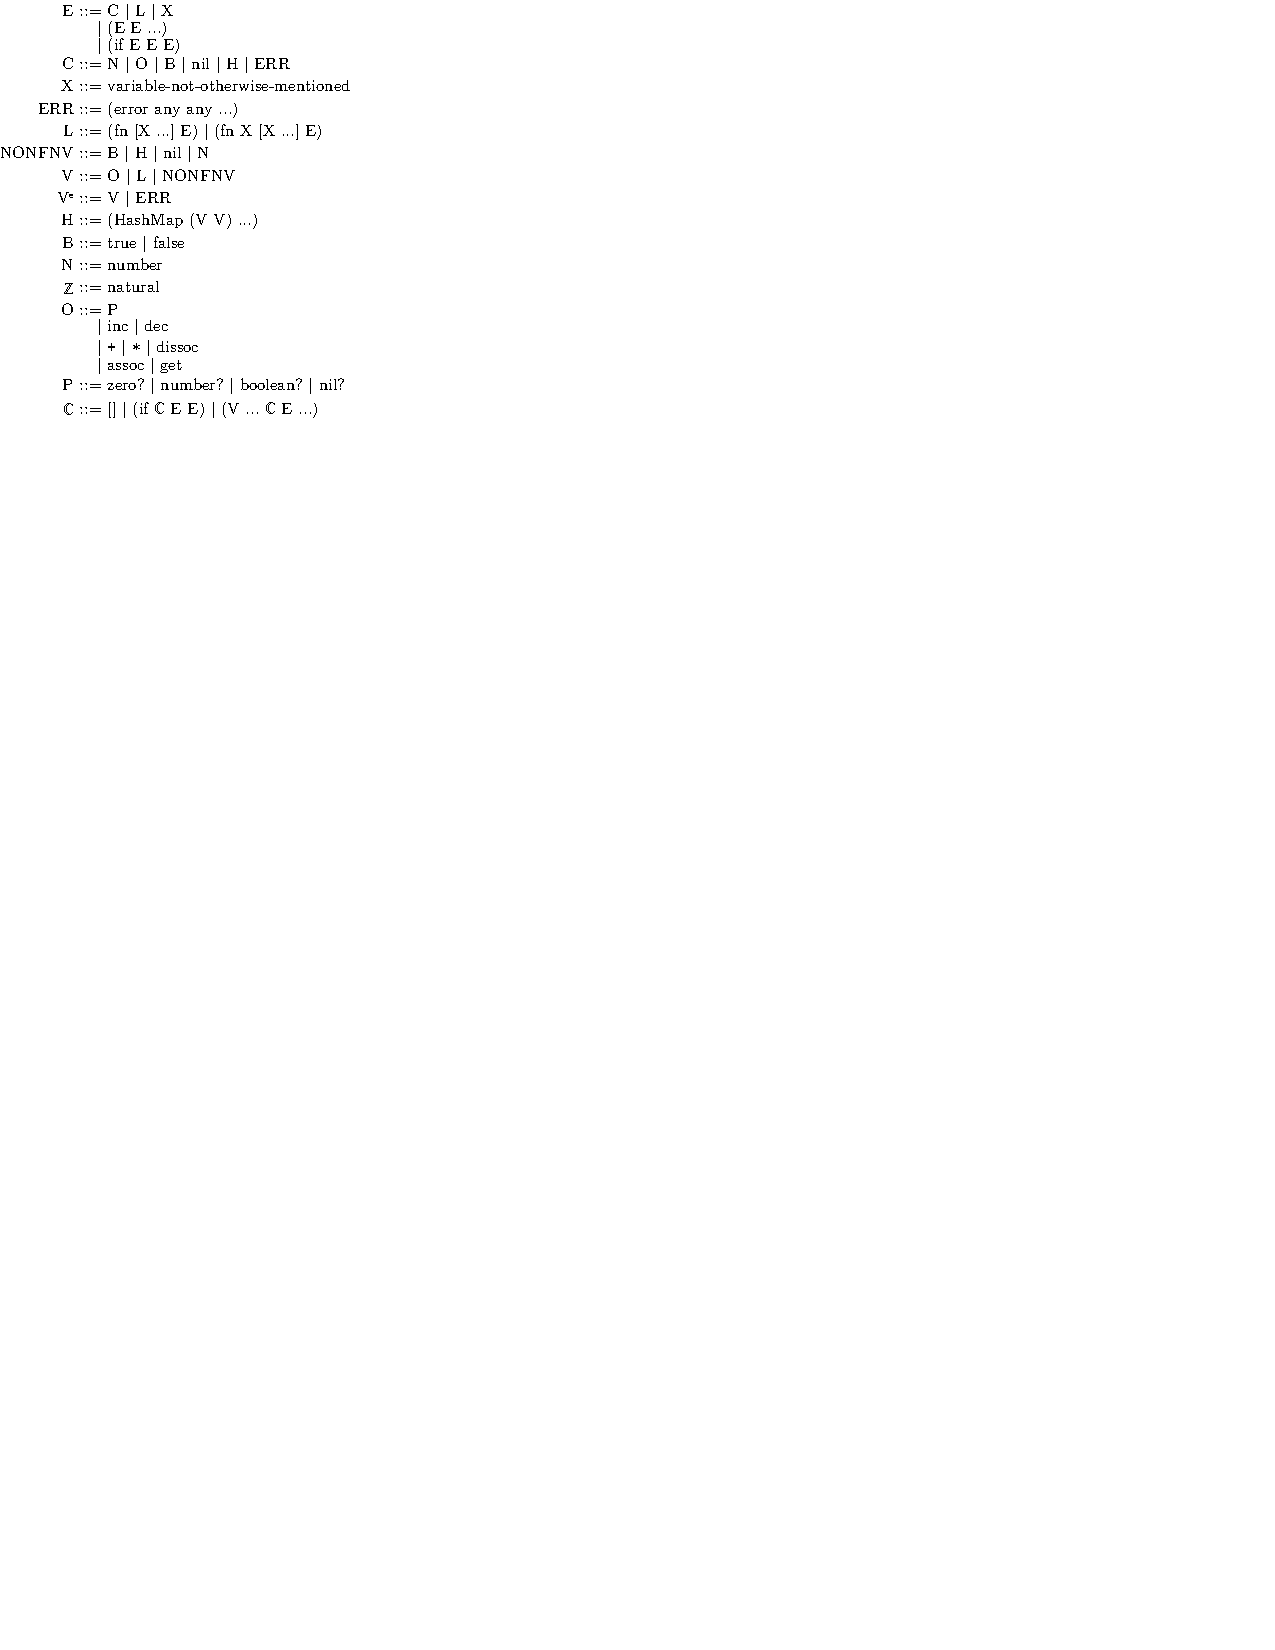
\includegraphics[]{redex/clojure-grammar.pdf}
}
\caption{Syntax of Terms in $\lambda c$.
  Expressions \texttt{E} consist of (loosely named) ``constant'' expressions \texttt{C}
  (numbers \texttt{N}, built-in functions \texttt{O}, booleans, nil, hash maps \texttt{H}, and errors
\texttt{ERR}), 
  functions \texttt{L} (non-recursive, and recursive), variables \texttt{X}, applications,
  and conditionals.
  The built-ins \texttt{assoc}, \texttt{dissoc}, and \texttt{get} perform the
  hash map operations add, remove, and lookup, respectively.
  Values are denoted \texttt{V}, and we use contexts $\mathbb{C}$ to define reduction rules.
  }
  \label{clojure-grammar}
\end{figure*}

%\begin{figure*}
$$
\begin{altgrammar}
  \e{} &::=& ... \alt &\mbox{Expressions} \\
\end{altgrammar}
$$
\caption{Syntax of $\lambda c_s$ (extending $\lambda c$)}
\end{figure*}


\begin{figure*}
\fbox{
  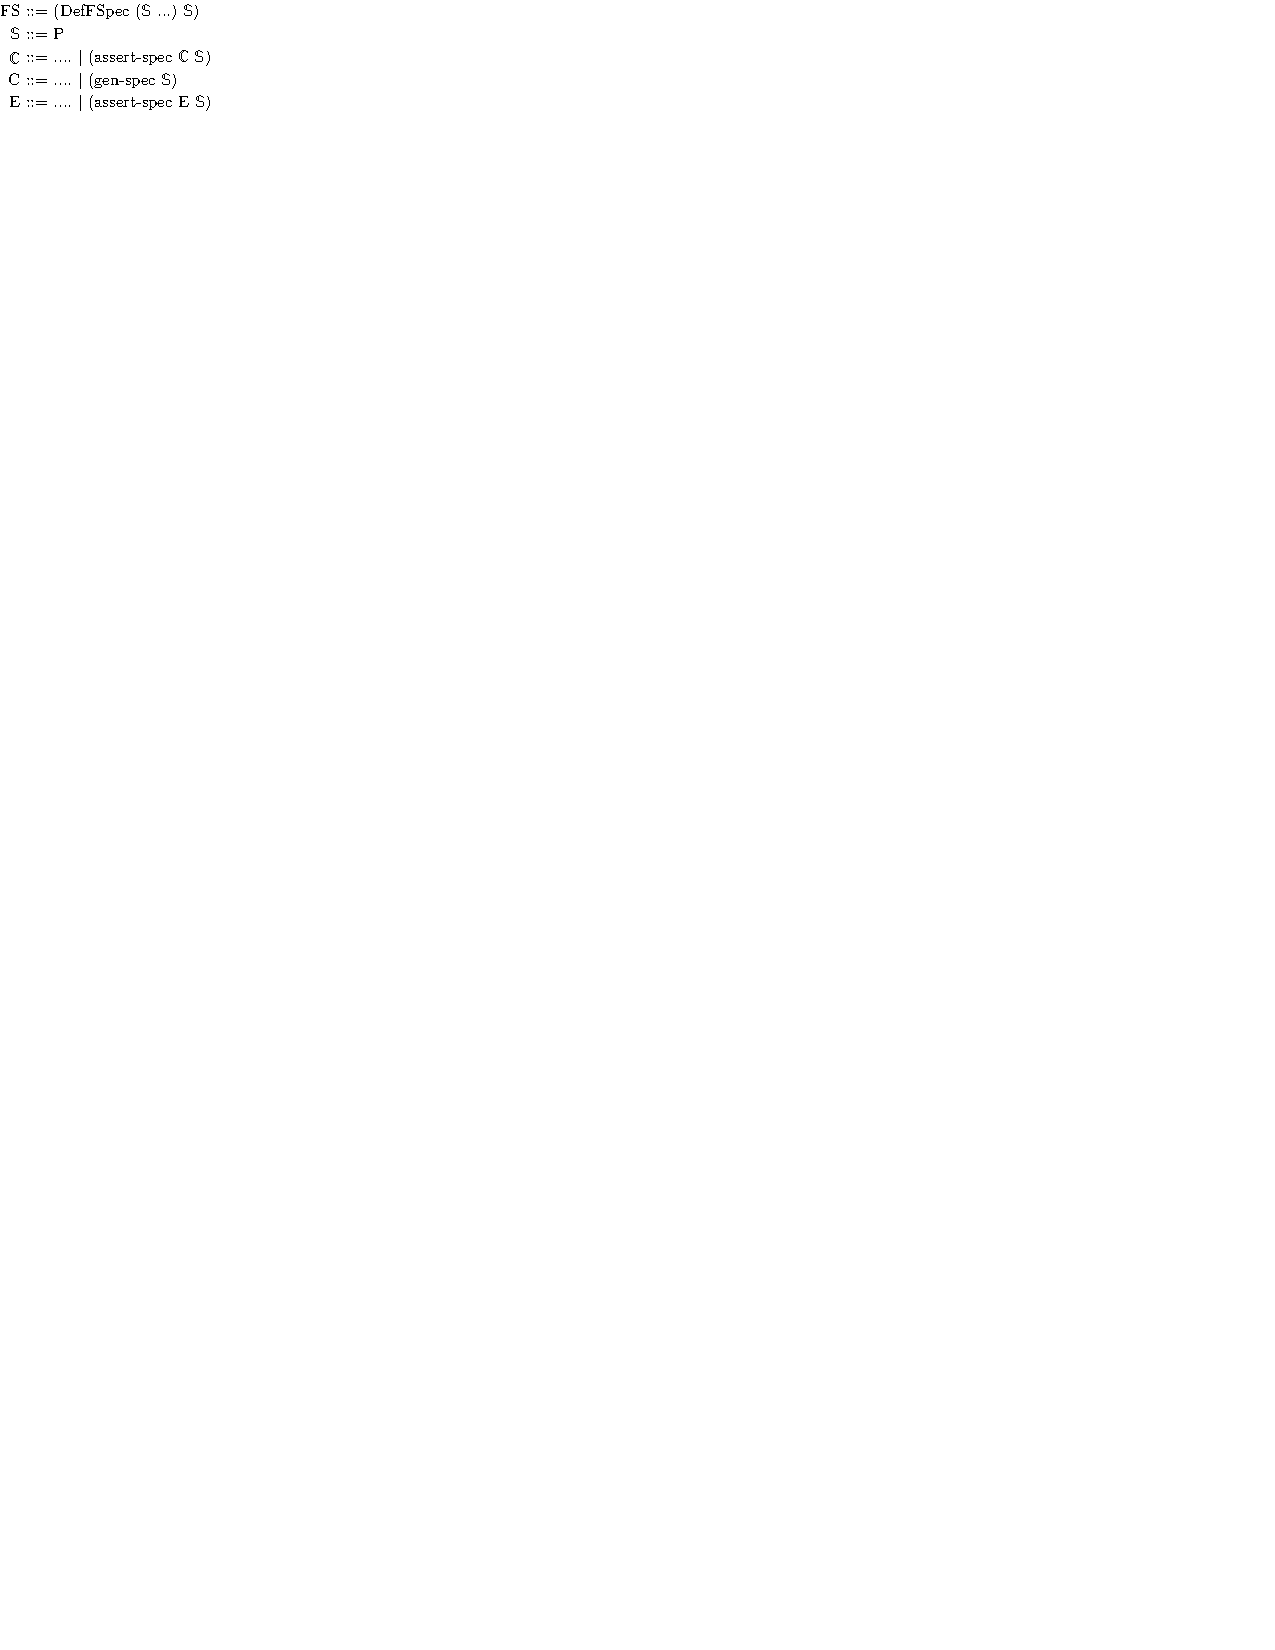
\includegraphics[]{redex/clojurespec-grammar.pdf}
}
\caption{Syntax of $\lambda c_s$ (extending $\lambda c$).
  We add the \texttt{assert-spec} form that takes an expression and a spec
  and checks the expression evaluates to a value conforming to the spec.
  We restrict specs to just predicates \texttt{P}.}
  \label{clojurespec-grammar}
\end{figure*}

%\begin{figure*}
$$
\begin{altgrammar}
  \e{} &::=& ... \alt &\mbox{Expressions} \\
\end{altgrammar}
$$
\caption{Syntax of $\lambda c_s^f$ (extending $\lambda c_s$)}
\end{figure*}

\begin{figure*}
\fbox{
  
\includegraphics[]{redex/clojurespechof-grammar.pdf}
}
\caption{Syntax of $\lambda c_s^f$ (extending $\lambda c_s$).
  We add two forms of \texttt{fspec}s---the natural number represents how
  many times to generatively test a function value.
  }
  \label{clojurespechof-grammar}
\end{figure*}

\begin{figure}
\fbox{
  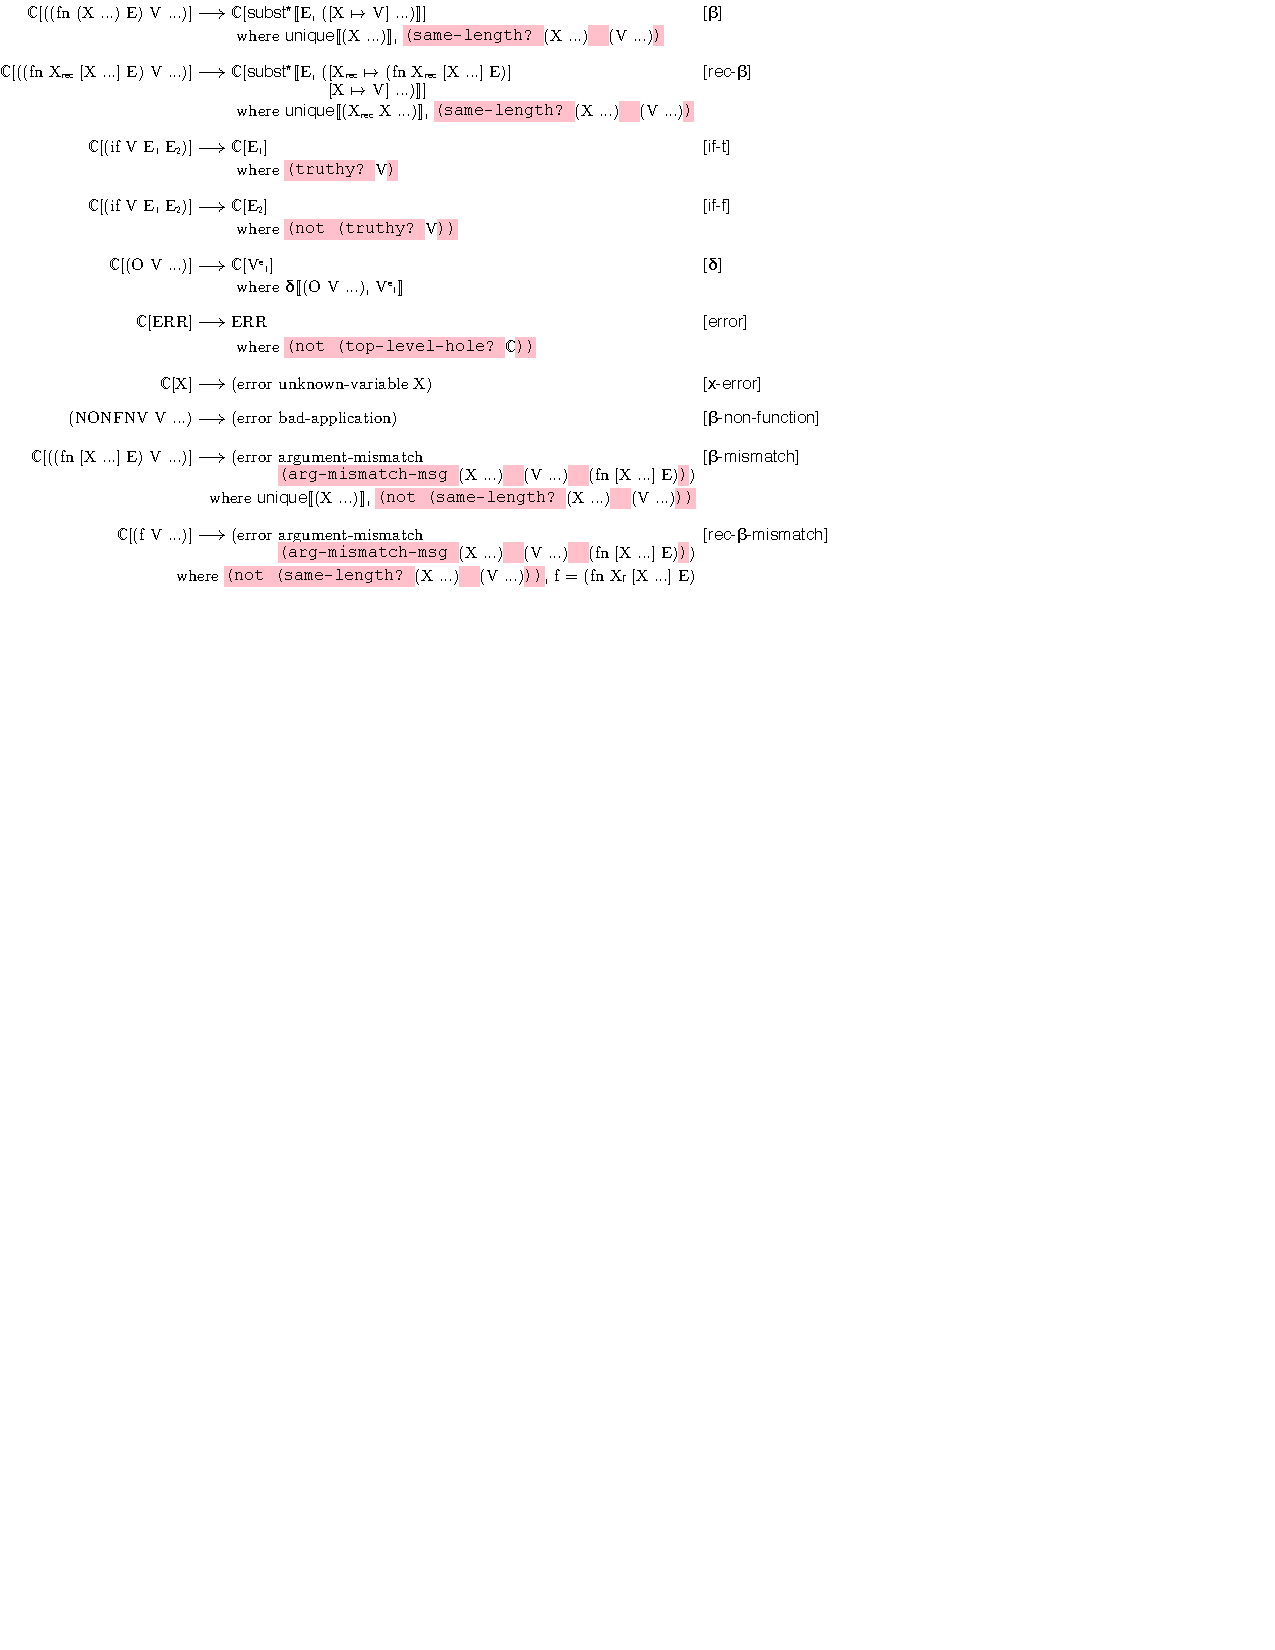
\includegraphics[]{redex/arrowv.pdf}
}
\caption{Small-step reduction relation in $\lambda c$.
  We define $\beta$ reduction rules for both types of functions.
  Then branching rules for conditionals (\texttt{false} and \texttt{nil} are false values),
  and constant functions ($\delta$, full definition omitted).
  Finally several rules for throwing detailed runtime errors.
  }
  \label{arrowv}
\end{figure}

\begin{figure*}
\fbox{
  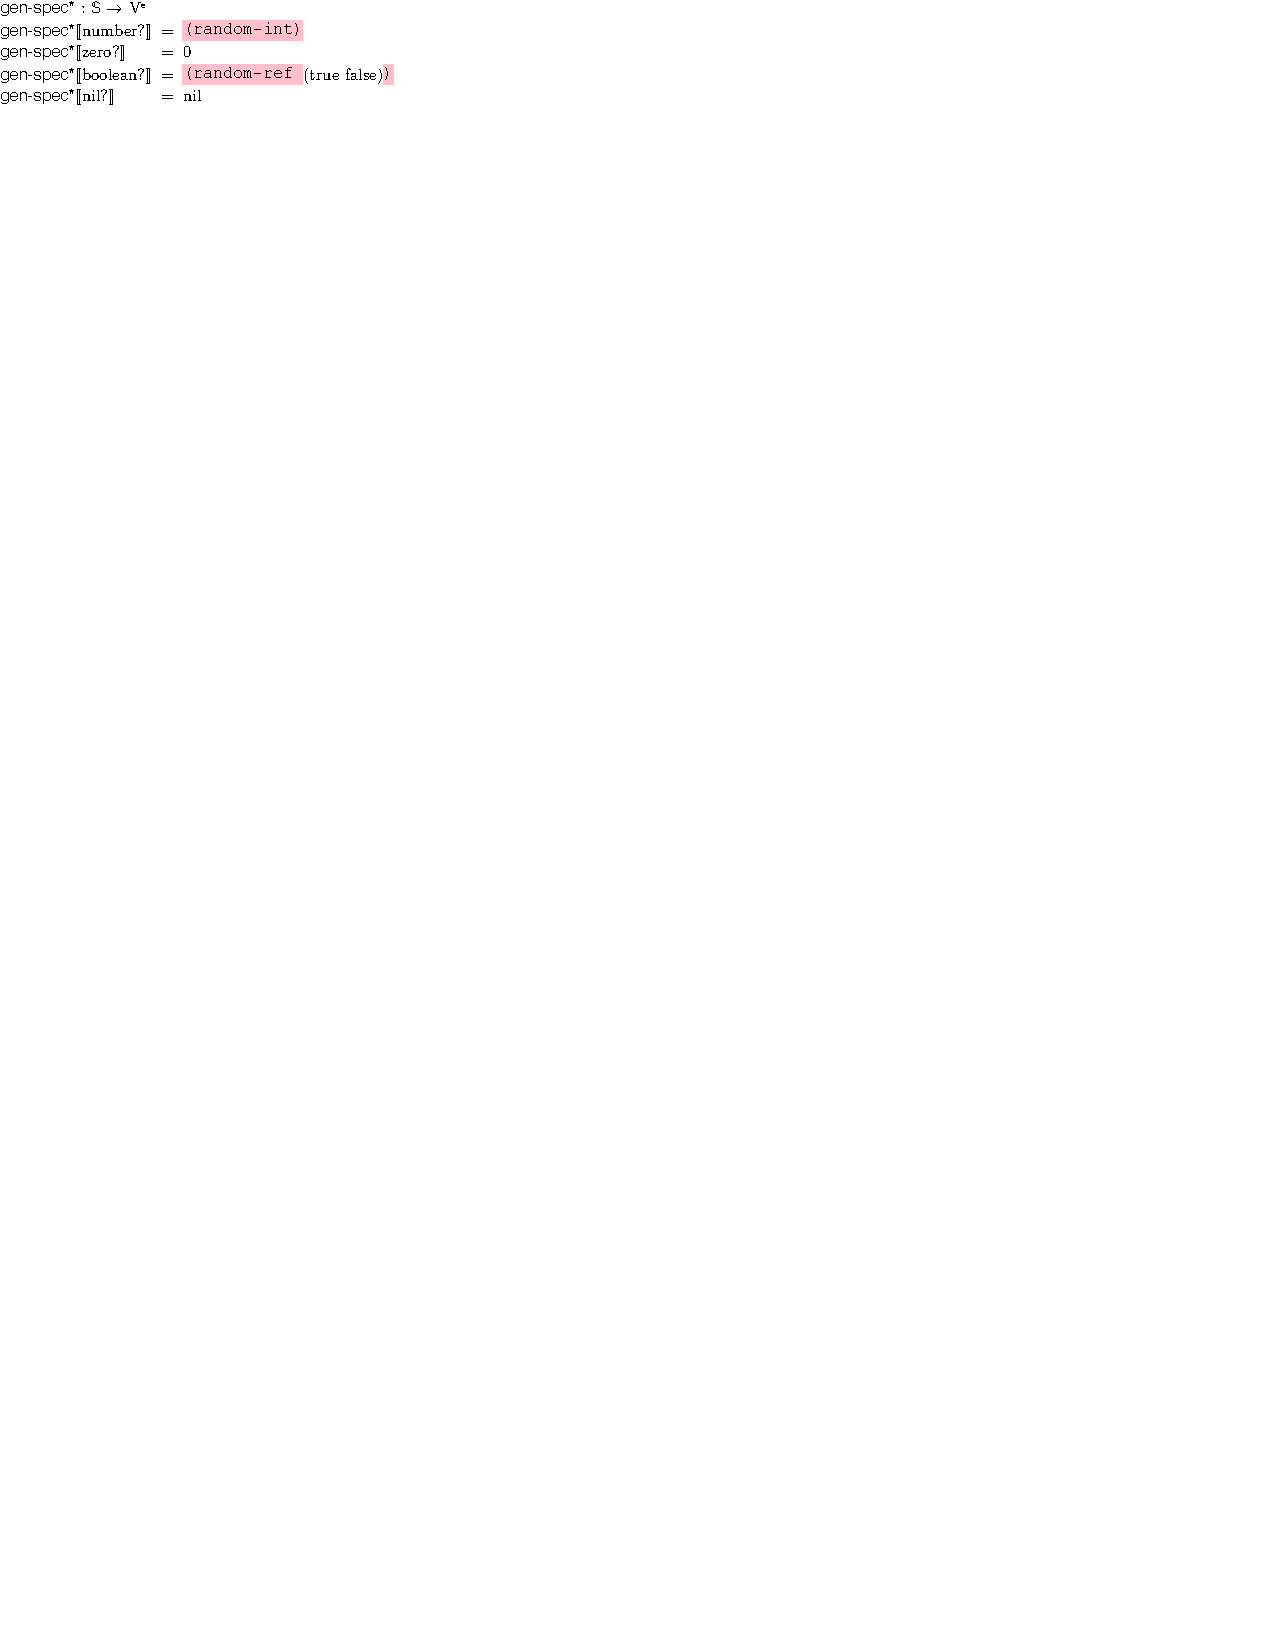
\includegraphics[]{redex/gen-spec*.pdf}
}

\fbox{
  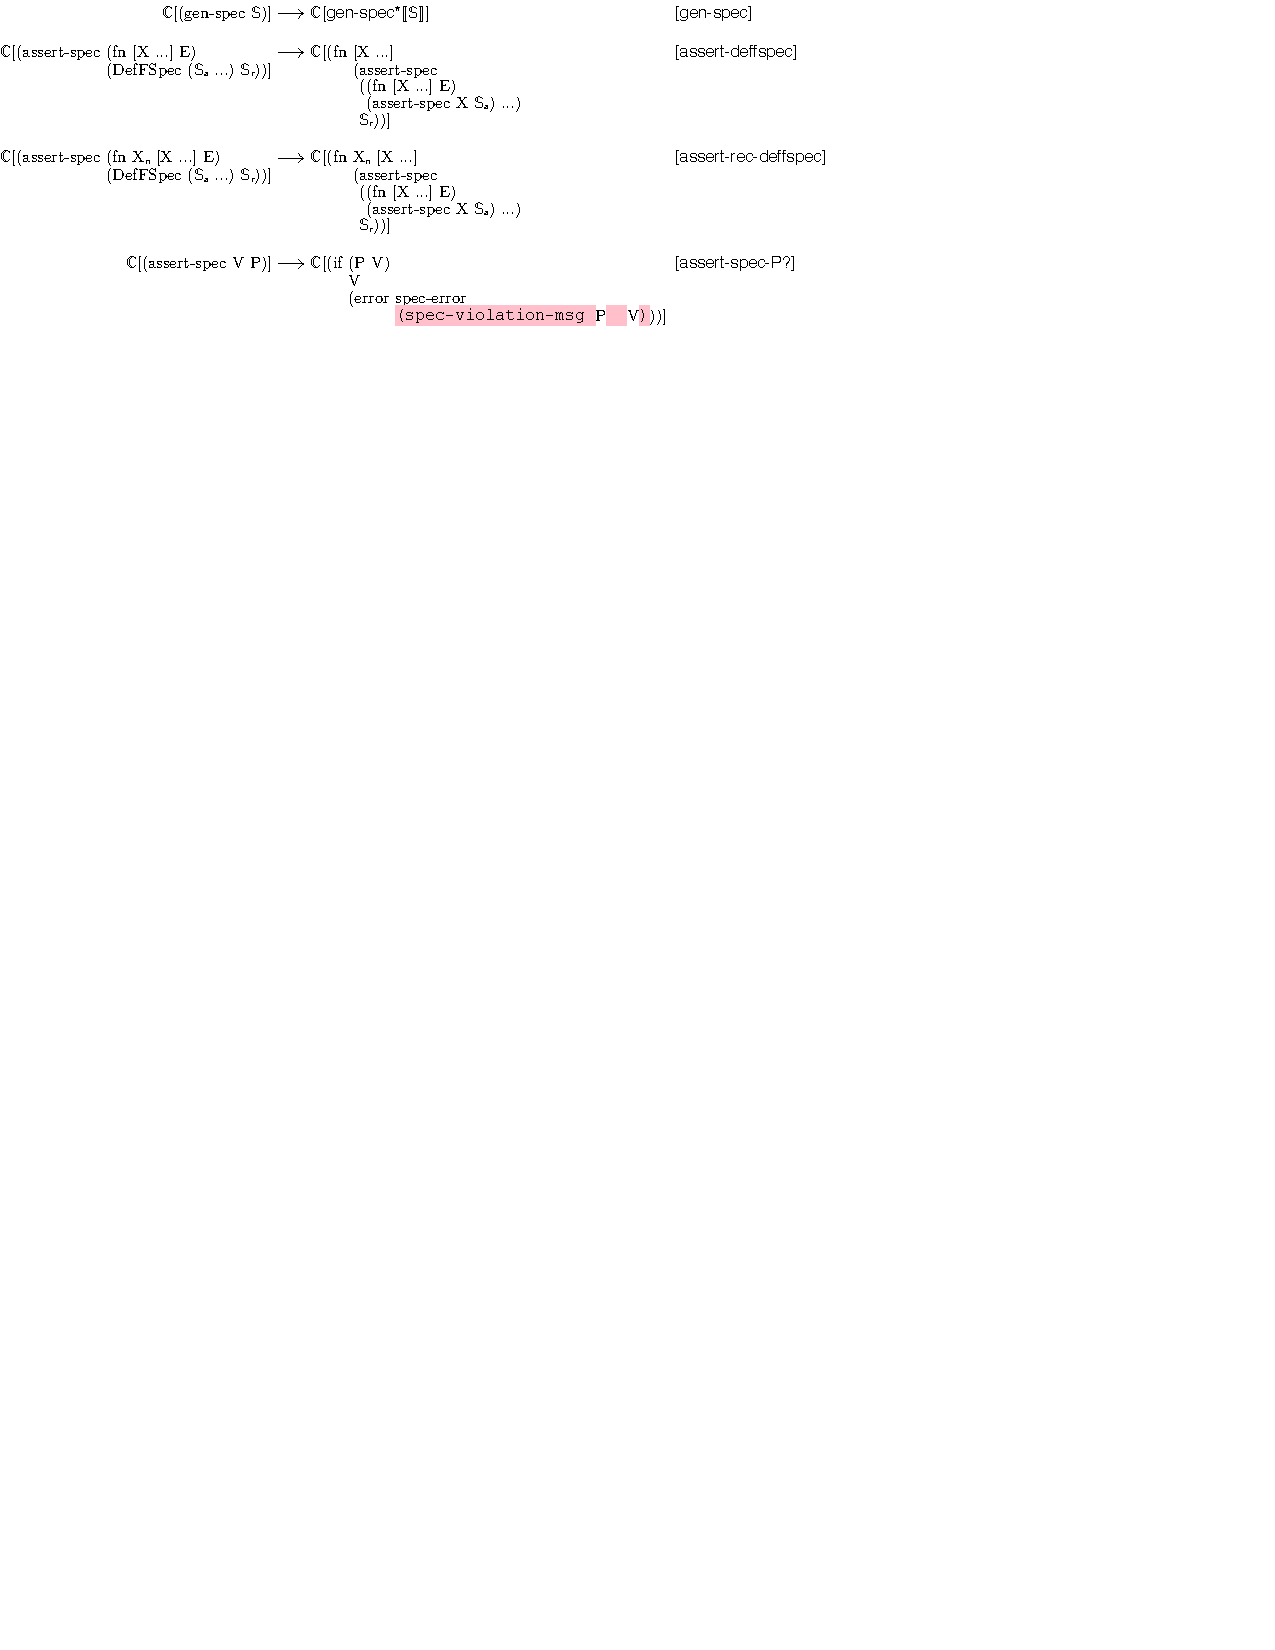
\includegraphics[]{redex/arrowvspec.pdf}
}
\caption{Small-step reduction relation in $\lambda c_s$ (extending $\lambda c$).
  \texttt{gen-spec} takes a spec and generates a value conforming to that spec
  via the \texttt{gen-spec*} metafunction.
  We define \texttt{assert-spec} with support for 
for \texttt{fdef} using traditional proxy checking semantics, and flat predicates.}
  \label{arrowvspec}
\end{figure*}

\begin{figure*}
\fbox{
  
\includegraphics[]{redex/gen-spec*-hof.pdf}
}

\fbox{
  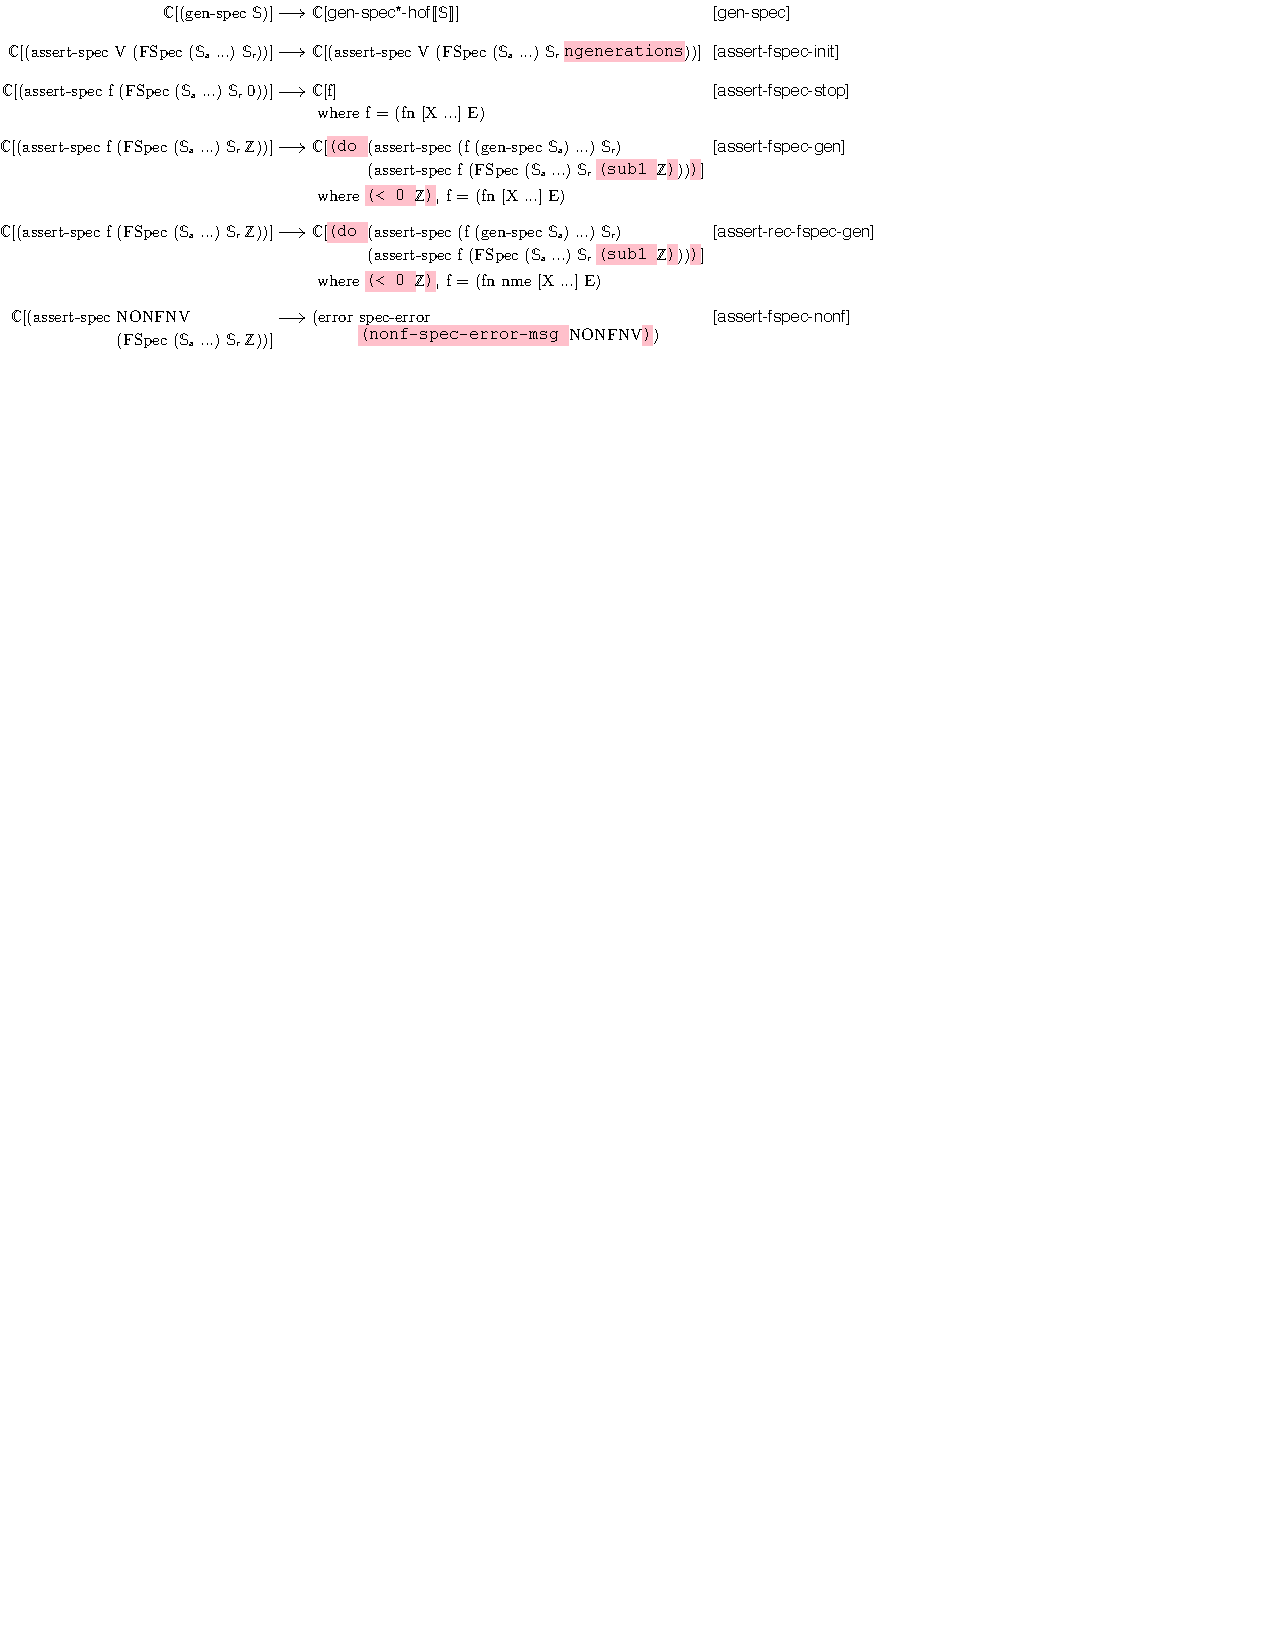
\includegraphics[]{redex/arrowvspec-hof.pdf}
}
  \caption{Small-step reduction relation for $\lambda c_{s}^{f}$ (extending $\lambda c_s$)
  \texttt{gen-spec} takes a spec and generates a value conforming to that spec
  via the \texttt{gen-spec*-hof} metafunction (which extends \texttt{gen-spec*} in Figure~\ref{arrowvspec}).
  }
  \label{arrowvspec-hof}
\end{figure*}
